\subsubsection{LoG算子}
高斯算子取图像的周围几个像素取平均值,这样就能实现模糊图像,去除噪声的作用。
保留了图片的大致特征,就像人眯起眼睛看东西或者从不同距离看东西一样。

$\sigma$表示高斯核的大小,$\sigma$越大,则经过高斯卷积的图像越模糊。不同$\sigma$处理的图像就形成了一个三维的\textbf{尺度空间}。

\begin{figure}[h]
    \centering
    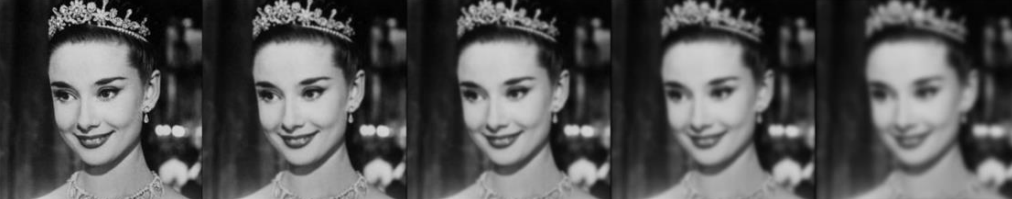
\includegraphics[height=1in]{LoG.png}
    \caption{尺度空间}
    \label{fig:harrisShape}
\end{figure}

对不同尺度下的图像求二阶导数,并取极值点,就得到了LoG算子:
\begin{equation*}
    \nabla^2L(x, y, \sigma_D)=(\frac{\partial^2L(x,y,\sigma_D)}{\partial x^2} + \frac{\partial^2L(x,y,\sigma_D)}{\partial y^2})*I(x,y)
\end{equation*}

尺度归一化LoG算子:

\begin{equation*}
    \nabla_{norm}^{2}L(x, y, \sigma_D)=\sigma_{D}^{2}(\frac{\partial^2L(x,y,\sigma_D)}{\partial x^2} + \frac{\partial^2L(x,y,\sigma_D)}{\partial y^2})*I(x,y)
\end{equation*}

不同尺度下的LoG响应值不具有可比性

\begin{figure}[h]
    \centering
    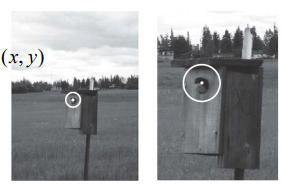
\includegraphics[height=1in]{不同尺度LoG极值点.png}
    \caption{不同尺度LoG极值点}
    \label{fig:harrisShape}
\end{figure}

需要计算位置空间和尺度空间寻找归一化LoG极值,作为特征点。

LoG特征检测结果效果好,但是计算量很大。(每个像素)
\begin{figure}[h]
    \centering
    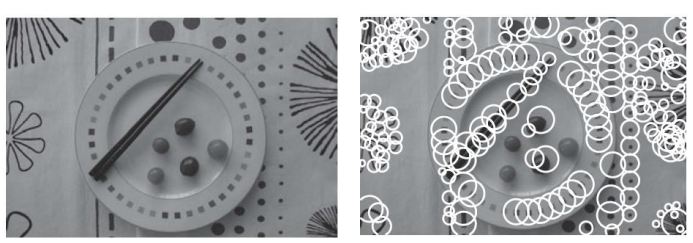
\includegraphics[height=2in]{LoG效果.png}
    \caption{LoG效果}
    \label{fig:harrisShape}
\end{figure}